This appendix supplements the main paper. It records
configuration and provenance separately from the main scientific argument.

\section{Training, decoder and runtime configuration}\label{training-decoder-and-runtime-configuration}

\begin{longtable}[]{@{}
  >{\raggedright\arraybackslash}p{(\linewidth - 2\tabcolsep) * \real{0.5000}}
  >{\raggedright\arraybackslash}p{(\linewidth - 2\tabcolsep) * \real{0.5000}}@{}}
\toprule\noalign{}
\begin{minipage}[b]{\linewidth}\raggedright
Item
\end{minipage} & \begin{minipage}[b]{\linewidth}\raggedright
Executed configuration
\end{minipage} \\
\midrule\noalign{}
\endhead
\bottomrule\noalign{}
\endlastfoot
Frozen PLM & ESM2-35M, \nolinkurl{esm2_t12_35M_UR50D}, layer12,480 channels \\
Frozen folding model & \nolinkurl{protenix_mini_default_v0.5.0} \\
Official system & \nolinkurl{protenix_mini_esm_v0.5.0}, ESM2-3B native single-sequence route \\
Interface & Single Mini OPM boundary; subsequent MSA pair stack retained \\
Query input & One-hot query profile, zero deletion features; no homolog/template inputs \\
Decoder & \(G_D(a,b)=[D W\operatorname{vec}(a\otimes b)+b_{out}]/(D+0.001)\) \\
Student depth & 508.5, existing Train24 median, fixed scalar at inference \\
Native factor width / pair channels & 32 /128 \\
Encoder & Independent copies of projection/CNN/global encoder, hidden128; paired equal initialization \\
Trainable parameters & Factor373,824; Generic378,272; G+378,144 \\
Task optimizer & AdamW; weight decay\(10^{-4}\); global gradient norm clip1 \\
Original four-cell task learning rate & \(10^{-4}\);384 updates \\
G+ search & Each head:\(5\times10^{-5},10^{-4}\);3 seeds per LR;384 updates \\
G+ selected learning rates & Factor\(5\times10^{-5}\); G+\(10^{-4}\) \\
Budget extension & Restore full AdamW state; total768/1536 evaluation;1536 ceiling \\
Recycles / backward & 4; final recycle retains gradients; backbone weights frozen \\
Task noise draws & 1 per target update; \(\sigma=16\exp(-1.2+1.5z)\), \(z\sim N(0,1)\) \\
Coordinate training & Native rigid augmentation, noisy true coordinates, single denoiser call \\
Denoiser conditioning & \nolinkurl{use_conditioning=True}; condition embedding drop rate0 \\
Confidence conditioning dropout & 0; confidence loss disabled \\
Training dropout configuration & MSA pair stack pair dropout0.25; Pairformer dropout0.25; model in train mode \\
MSA dropout configuration & 0.15 configured, but native MSA embedding/OPM path is replaced by injected update \\
Monte Carlo inference dropout & Apply rate0 and dropout rate0; model in eval mode \\
Numeric mode & FP32; loss and diffusion paths outside AMP \\
Structure inference & c4/s5;1 sample; seed 101; no ground-truth-based selection \\
UT optimizer & AdamW,\(2\times10^{-4}\), weight decay\(10^{-4}\);1,000 steps \\
UT sampling & 4,096 ordered pairs including diagonal; same sampled pairs across paired heads \\
UT scale & Train24 per-channel standard deviation, floor\(10^{-3}\); scale errors only \\
UT target & \(P_Q\) profile/deletion conditions, true fixed MSA factors, actual per-target depth \(N_i\), final reconstructed marginal update \\
Stage transition & Reset optimizer between U distillation and task training; no reset during budget continuation \\
\end{longtable}

\subsection{Native loss details}\label{native-loss-details}

The configured task objective is

\[
\mathcal L_{task}=4\mathcal L_{MSE}+4\mathcal L_{bond}
+4\mathcal L_{smooth-lDDT}+0.03\mathcal L_{distogram}.
\]

The native MSE term includes its internal factor 1/3, coordinate observation
mask, weighted rigid alignment, and noise-dependent scale
\((\sigma^2+16^2)/(16\sigma)^2\). Protein atom weights are1; configured DNA/RNA
weights 5 and ligand weights 10 do not affect these protein-only examples.
Loss numerical epsilons are\(10^{-6}\). The distogram uses 64 bins, with configured
minimum 2.3125Å and maximum 21.6875Å. Native smooth-lDDT is a training loss and
is distinct from the reported reference-masked Cα distance metric.

All 30 saved reports across the original four-cell, explicit-access and budget
studies use the same loss configuration. \textbf{Every recorded task update has
\nolinkurl{bond_mask_count=0}}: the configured bond coefficient is nonzero, but this term
contributes zero on these inputs. Confidence weight is 0. These findings come
from actual saved reports and installed source, not unmodified library defaults.
The extraction is retained in configuration\_audit.json (\nolinkurl{configuration_audit.json}).

\subsection{Hardware, software and concurrency}\label{hardware-software-and-concurrency}

Experiments ran on AMD MI250 hardware, exposed as 8 GPU devices/GCDs
with approximately 64GiB per device. There was one training process per assigned
GPU. The original four-cell launch used up to 8 devices; G+ search and budget
continuation used 6 workers. Independent96 inference used 8 workers, scheduling
14 fixed model instances. These concurrent-device measurements are specific
to this runtime and workload; no standalone universal latency is implied.

\begin{longtable}[]{@{}ll@{}}
\toprule\noalign{}
Runtime component & Recorded version / setting \\
\midrule\noalign{}
\endhead
\bottomrule\noalign{}
\endlastfoot
Python & 3.12 \\
Protenix & 1.1.0 installed wheel \\
PyTorch & 2.12.0a0+git78258b9 \\
HIP & 7.14.60850 \\
fair-esm & 2.0.0 \\
Biopython & 1.88 \\
LayerNorm backend & \nolinkurl{LAYERNORM_TYPE=torch} \\
CPU threading & \nolinkurl{OMP_NUM_THREADS=4} for folding/training workers \\
\end{longtable}

The exact installed Protenix wheel-to-upstream-commit mapping is not established;
checkpoint hashes, installed versions and experiment source snapshots are retained
instead of claiming a verified upstream revision.

\section{Panel selection and research chronology}\label{panel-selection-and-research-chronology}

The96-target panel was selected from an existing pre-2021-09-30 catalog without
opening the parent project's reserved temporal-test manifests or post-cutoff
coordinates. All target sequences were checked against the 32 prior adaptation/
development queries and 15,053 distinct old query/MSA sequences. The alignment
is global: match2, mismatch-1, gap-open-8, gap-extend-1, first optimal alignment.
A near-homology exclusion requires ≥50 paired columns and≥30\% identity among
paired columns, with the coverage rule below. One PDB is allowed per panel.

Version1 required≥70\% coverage of the shorter sequence for query, MSA-row and
within-panel comparisons. It exhausted 11,423 candidates in the shortest stratum
with 14/24 accepted and stopped without panel predictions. Before any new panel
prediction or scoring, version2 changed \textbf{only the MSA-row rule} to≥70\% coverage
of candidate length. Query and within-panel rules kept the shorter denominator;
a sequence shared by query/MSA retains the stricter query rule. Length quotas,
ranking, model selection and scoring stayed fixed.

Version2 filled all 96 slots from 434 examined records:96 accepted,263 similarity
exclusions,30 mapping failures and45 within-panel homolog exclusions. Ranking
used SHA256 of \texttt{engramfold-independent96-v1\textbar{}\textless{}target\_id\textgreater{}}. Exact sequence mapping
used entity\_poly\_seq and model1 label\_seq\_id; finite observed Cα coverage was
required to be≥90\%. Manifest SHA256:
\nolinkurl{702d8b73d196cb5351ceb29b818737f6f62001a5a219db05445f2439f609fdde}.

The earlier Dev8 four-cell primary comparison was UT Factor-Generic and failed
its gate; a conditional bilinear experiment was not launched. A separately
declared study then froze existing checkpoints and made task-only Factor-Generic
the unique primary endpoint on the new96 panel. The earlier failed gate remains
failed. G+ and budget diagnostics were developed later and have no new independent
confirmation. This chronology prevents transferring the 96-target interval to
new checkpoints or controls.

A subsequent score-blind sequence audit retained all 96×32 old-query comparisons
and 4,560 within-panel pairs. Maximum identity to Train24/Dev8 among qualifying
coverage/paired-column alignments was28.24\%/27.72\%. At 20\%/25\%/30\% identity,
connected-component counts were 1/39/96. At 25\%, the largest component contained 56
chains; component-resampled chain-weighted mean differences had interval
{[}0.05092,0.09582{]}. At 20\%, one component cannot estimate between-component
uncertainty; a degenerate numeric interval is not valid evidence of precision.
These are threshold-defined sequence groups, not annotated families. No target
was removed on the basis of this audit.

\section{Scoring and implementation audit}\label{scoring-and-implementation-audit}

The original metric uses a fixed observed-reference Cα mask. Reference distances
must be\textgreater0 and\textless15Å; upper-triangular pairs avoid duplicates. Sequence neighbors
are retained; self-pairs are excluded. Error thresholds are strict\textless0.5,\textless1,\textless2,\textless4Å.
Missing predicted coordinates earn zero on all affected reference contacts,
without shrinking the denominator. This is Cα distance lDDT \citep{lddt}, not all-atom
lDDT with stereochemical corrections. Pair-global aggregation is a legitimate
variant; per-residue means apply different contact weighting.

All 1,344 CIF hashes, reference masks and target ordering were checked. The
AlphaFold lDDT source was pinned to
\nolinkurl{c77e5d2a8961d1a353632c462914ff0a32a950f6}. Its sole JAX import was replaced by
NumPy and FP64 coordinate inputs were used; this is a disclosed backend port,
not execution under native JAX. Scores match within 1.016e-14. The reference
implementation uses directed symmetric pairs and tiny numerical epsilons;
these do not materially change this panel's scores. All predictions cover the
fixed reference positions, so this agreement is not an independent validation
of missing-prediction behavior; the latter has separate unit tests.

Supplementary TM-score uses USalign/TMscore commit
\nolinkurl{fcb0f9d921415a2095bc509975db7fc1e968af1d}, compiled with \nolinkurl{g++\ -O3}.
CA-only PDB export preserves label\_seq\_id. Default residue-index correspondence
is retained, without \nolinkurl{-seq}; \texttt{-l\ \textless{}full\ query\ length\textgreater{}} sets normalization.
Rigid-body search is allowed; rematching residues is not. Unobserved reference
residues have no numerator contribution but remain in the length denominator.
Output precision is four decimals. Synthetic executable checks yield 1.0 for
rigid translation,0.5 for half missing residues and 0.121 for reversed numbering.
The earlier single-Kabsch auxiliary metric remains separately named.

All supplementary metrics are post-result sensitivity analyses, not replacement
primary endpoints. Official Mini-ESM scores were included in the same audit;
its high scores alone establish neither data leakage nor an implementation error.

\section{Complete development curves and costs}\label{complete-development-curves-and-costs}

\begin{figure}
\centering
\pandocbounded{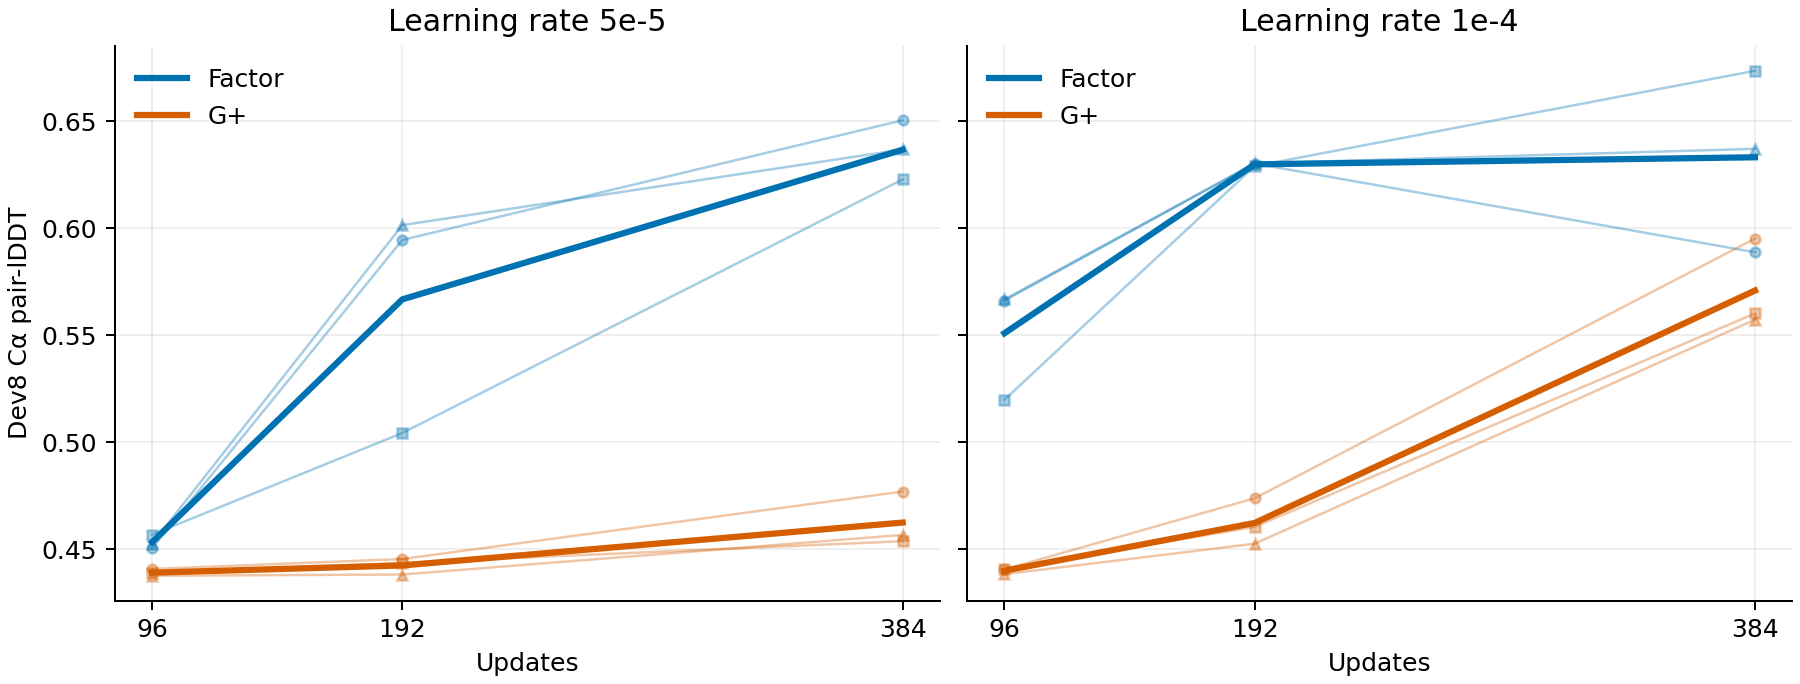
\includegraphics[keepaspectratio]{figures/factor_access_all_trials.png}}
\caption{All learning-rate trials}
\end{figure}

\textbf{Figure S1.} Both predeclared learning rates at 96/192/384, for both heads and
all three paired seeds. Each head selects its learning rate by final Dev8 mean,
not by the best seed or an earlier node. Width changes in G+ preserve approximate
parameter count, so this is not an isolated causal estimate of input access.

\begin{figure}
\centering
\pandocbounded{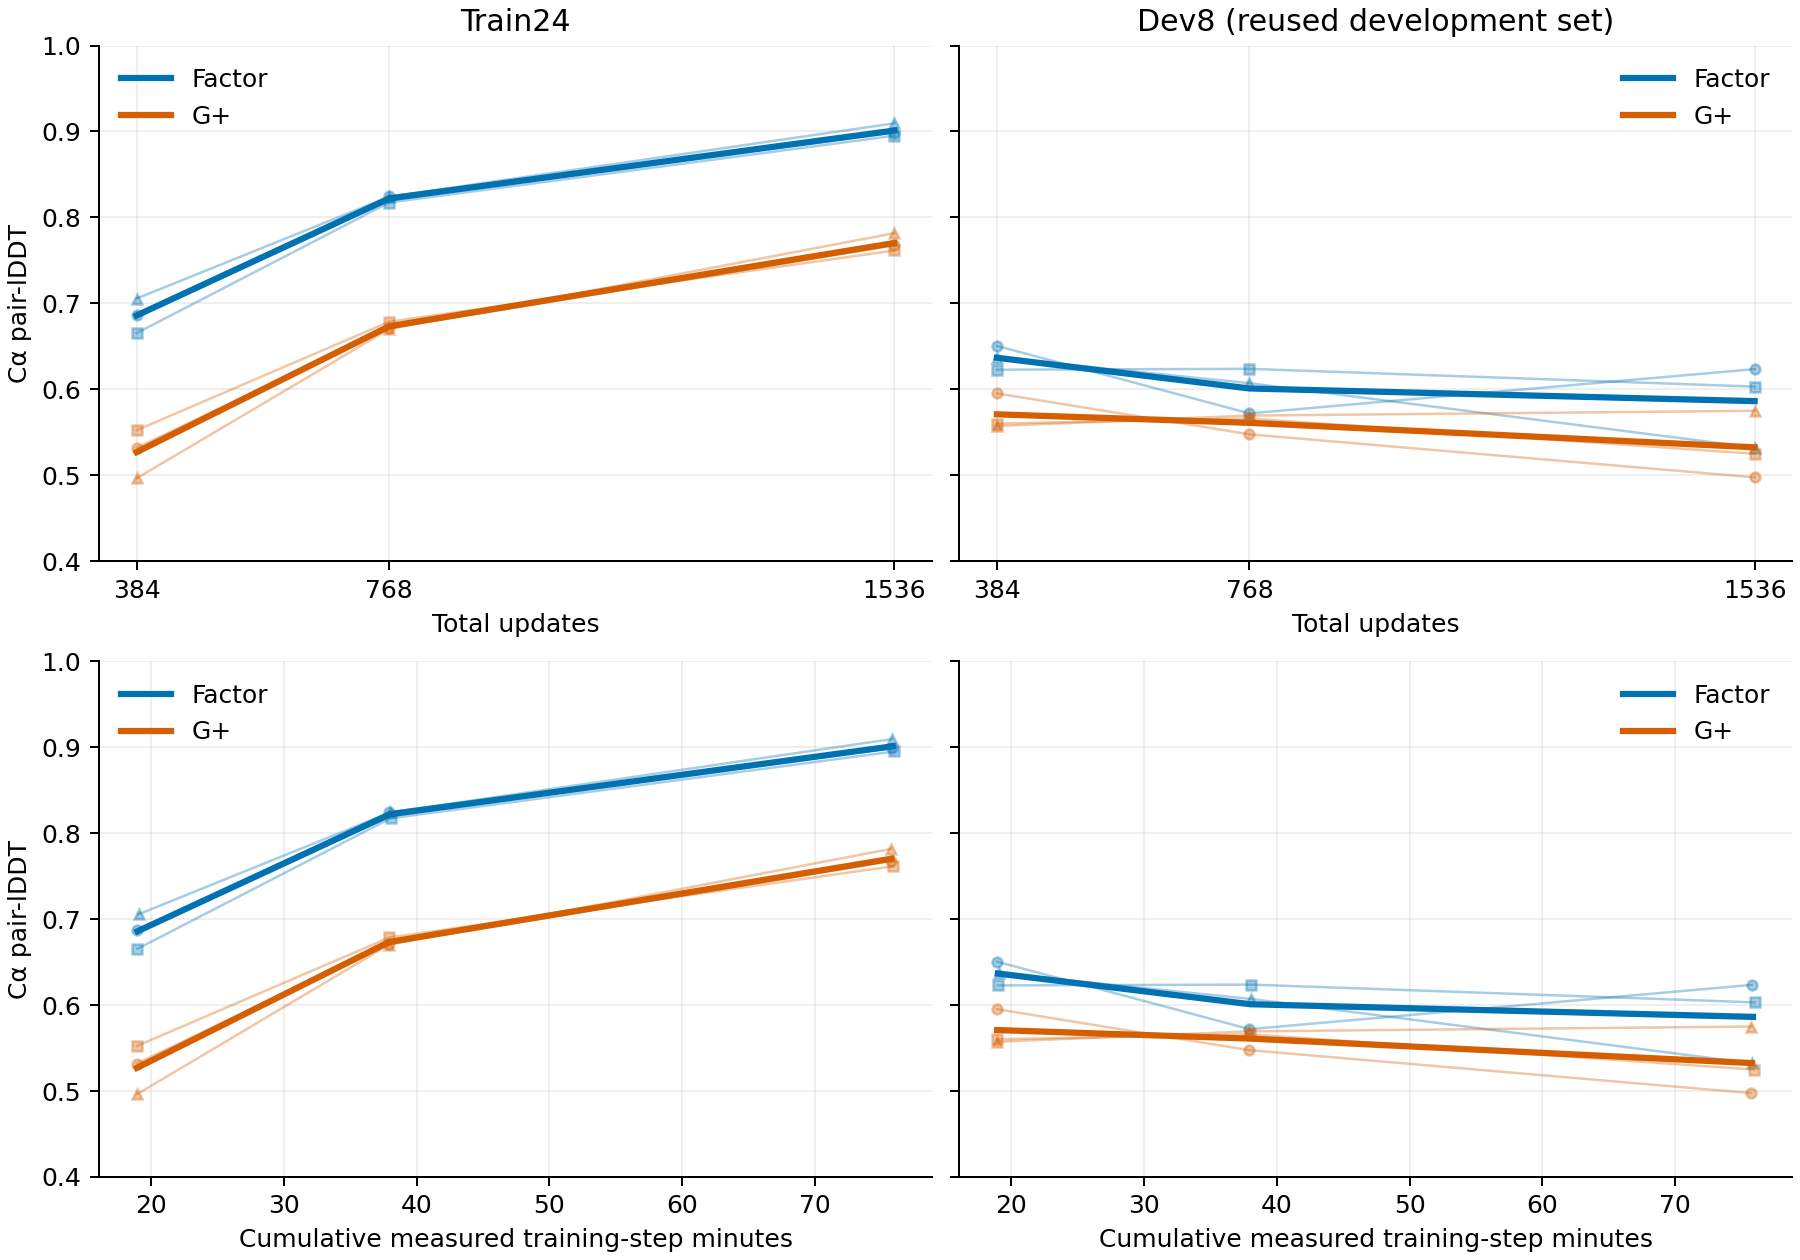
\includegraphics[keepaspectratio]{figures/budget_sensitivity.png}}
\caption{Complete budget sensitivity figure}
\end{figure}

\textbf{Figure S2.} Train24 and Dev8 at 384/768/1536 versus updates and cumulative
training-step minutes. Thin lines/markers represent paired seeds20260920/21/22;
thick lines are means. The time panels mainly re-express the update axis because
per-step runtimes are similar. Segments are visual connections, not observed
intermediate trajectories. All 36 plotted records are in the accompanying CSV.

\begin{longtable}[]{@{}
  >{\raggedright\arraybackslash}p{(\linewidth - 10\tabcolsep) * \real{0.1364}}
  >{\raggedleft\arraybackslash}p{(\linewidth - 10\tabcolsep) * \real{0.1818}}
  >{\raggedleft\arraybackslash}p{(\linewidth - 10\tabcolsep) * \real{0.1818}}
  >{\raggedleft\arraybackslash}p{(\linewidth - 10\tabcolsep) * \real{0.1818}}
  >{\raggedleft\arraybackslash}p{(\linewidth - 10\tabcolsep) * \real{0.1818}}
  >{\raggedright\arraybackslash}p{(\linewidth - 10\tabcolsep) * \real{0.1364}}@{}}
\toprule\noalign{}
\begin{minipage}[b]{\linewidth}\raggedright
Budget
\end{minipage} & \begin{minipage}[b]{\linewidth}\raggedleft
Factor Train24
\end{minipage} & \begin{minipage}[b]{\linewidth}\raggedleft
G+ Train24
\end{minipage} & \begin{minipage}[b]{\linewidth}\raggedleft
Factor Dev8
\end{minipage} & \begin{minipage}[b]{\linewidth}\raggedleft
G+ Dev8
\end{minipage} & \begin{minipage}[b]{\linewidth}\raggedright
Dev difference interval
\end{minipage} \\
\midrule\noalign{}
\endhead
\bottomrule\noalign{}
\endlastfoot
384 & 0.68594 & 0.52694 & 0.63674 & 0.57095 & {[}0.01677,0.11128{]} \\
768 & 0.82198 & 0.67337 & 0.60100 & 0.56104 & {[}-0.03013,0.10717{]} \\
1536 & 0.90108 & 0.77025 & 0.58629 & 0.53254 & {[}-0.01938,0.14222{]} \\
\end{longtable}

These intervals are descriptive and unadjusted for learning-rate selection and
repeated development use. Final seed differences are +0.12590,+0.07817,-0.04281.
Cumulative mean step-minutes for Factor/G+ are 18.99/18.94,38.01/37.92 and
75.87/75.78. Initial12-run search consumes 3.793 GPU-hours of measured steps;
continuation adds 5.686 GPU-hours. Startup, cache loading, checkpoint I/O and
scoring are excluded. These are not complete experiment wall-time estimates.

Independent96 synchronized inference stage means for Factor are 0.0217s PLM,
0.1248s adapter and2.0151s folding; official means are 0.0851s,0.0008s and2.0043s.
Their sums exclude CPU preparation (approximately0.39s) and startup. Base-model
load is approximately 21s; measured ESM35/ESM3B loads are 0.65049s/25.1665s.
Cached PLM features do not make cold feature generation free.

\section{Reproducibility and research provenance}\label{reproducibility-and-research-provenance}

Original seeds:20260917/18/19. G+ and continuation seeds:20260920/21/22.
The original heads start at exact query-only outputs with equal encoder copies.
Runtime audits verify frozen weights, live adapter gradients and retained pair
stack calls. Task noise resets to seed+step, while target order is reconstructed
from a local seed. Full optimizer-state restoration was verified by bitwise
comparison of uninterrupted versus paused/restarted updates385--386 for both heads.

A serialization-only issue in the earlier UT experiment was repaired and resumed
from saved optimizer/model states; original logs and source were retained. A
later G+ launch with a missing source manifest was stopped before development
scores, archived and restarted after sealing. No budgets were selected from
these implementation events. All final expected runs and evaluations completed.

The project initially explored conditional memory and feature-only prediction.
Those memory gates failed against independent Dense/capacity controls. These
results explain the research history but are not evidence for the current
factor adapter's success or for conditional memory. The method in the main
paper is memory-free. The initial additional-data feasibility audit was archived
without predictions. Subsequently authorized Train96 and Train384 studies are
reported separately below; the initial audit is not their evaluation.

\begin{longtable}[]{@{}
  >{\raggedright\arraybackslash}p{(\linewidth - 2\tabcolsep) * \real{0.5000}}
  >{\raggedright\arraybackslash}p{(\linewidth - 2\tabcolsep) * \real{0.5000}}@{}}
\toprule\noalign{}
\begin{minipage}[b]{\linewidth}\raggedright
Artifact
\end{minipage} & \begin{minipage}[b]{\linewidth}\raggedright
Location relative to repository
\end{minipage} \\
\midrule\noalign{}
\endhead
\bottomrule\noalign{}
\endlastfoot
Original frozen panel results/provenance & \nolinkurl{reports/independent_validation/} \\
G+ complete search, selected checkpoints & \nolinkurl{reports/query_factor_access/} \\
Fixed-budget continuation & \nolinkurl{reports/query_factor_budget/} \\
Scoring and sequence audit & \nolinkurl{reports/scoring_panel_audit/} \\
Exact four-cell protocol & \nolinkurl{docs/plm_interface_control_v1.md} \\
Panel protocol/amendment & \nolinkurl{docs/independent_validation_v1.md}, \nolinkurl{v2.md} \\
Explicit access/budget protocols & \nolinkurl{docs/query_factor_access_v1.md}, \nolinkurl{docs/query_factor_budget_extension_v1.md} \\
Plot generators & \nolinkurl{scripts/plot_paper_main.py}, \nolinkurl{scripts/plot_paper_budget.py} \\
Current configuration extraction & \nolinkurl{paper/configuration_audit.json} \\
\end{longtable}

Large checkpoints and original CIFs remain in the experiment artifact store. Sealed source snapshots, execution locks,
manifest/checkpoint/source hashes and raw per-target records preserve provenance.
The parent project's reserved temporal test and implementation were not modified.

\section{Native-direction96 numerical controls and scoring audit}\label{native-direction96-numerical-controls-and-scoring-audit}

The new protocol is native\_direction96\_v1 (\nolinkurl{docs/native_direction96_v1.md}). Train96 is the nested adaptation set; Confirm96-B is the new confirmation panel. It is distinct from the previously observed Confirm96-A. Target selection precedes all new predictions; confirmation is selected before training additions, which are then excluded against it. Sequence filters do not guarantee distant-family or foundation-pretraining isolation.

At matched writer states, all three rotations preserve exact query-only initialization. The following errors use the stored FP32 rotation matrices, with orthogonality and decoder-Gram checks accumulated in FP64. Residual checks use FP32 model arithmetic on one old training target, with a fixed nonzero head perturbation. They are numerical checks, not evidence of invariance along learned trajectories.

\begin{longtable}[]{@{}
  >{\raggedright\arraybackslash}p{(\linewidth - 6\tabcolsep) * \real{0.2000}}
  >{\raggedleft\arraybackslash}p{(\linewidth - 6\tabcolsep) * \real{0.2667}}
  >{\raggedleft\arraybackslash}p{(\linewidth - 6\tabcolsep) * \real{0.2667}}
  >{\raggedleft\arraybackslash}p{(\linewidth - 6\tabcolsep) * \real{0.2667}}@{}}
\toprule\noalign{}
\begin{minipage}[b]{\linewidth}\raggedright
Rotation seed
\end{minipage} & \begin{minipage}[b]{\linewidth}\raggedleft
max abs orthogonality error
\end{minipage} & \begin{minipage}[b]{\linewidth}\raggedleft
relative decoder Gram error
\end{minipage} & \begin{minipage}[b]{\linewidth}\raggedleft
max relative residual-norm error (full/tangent)
\end{minipage} \\
\midrule\noalign{}
\endhead
\bottomrule\noalign{}
\endlastfoot
20261001 & 2.573e-08 & 2.548e-08 & 6.370e-06 \\
20261002 & 2.818e-08 & 2.505e-08 & 3.114e-06 \\
20261003 & 1.991e-08 & 2.544e-08 & 2.787e-06 \\
\end{longtable}

All4,224 predictions were audited against the pinned AlphaFold lDDT implementation (NumPy substitution) and the previously pinned USalign TMscore executable. Fixed observed reference residues are retained, with full query-length TM normalization; residual mapping is not optimized. All predictions cover the reference residues. Maximum pair-lDDT discrepancy is1.216e-14. Primary supplementary contrasts and full system scores are preserved in metric\_audit.json (\nolinkurl{reports/native_direction96_20260919/metric_audit.json}). The post-result paired data×budget interaction is labeled supplementary in budget\_data\_interaction.json (\nolinkurl{reports/native_direction96_20260919/budget_data_interaction.json}). Neither alters the original primary gate.

\section{Native-direction extension: observed-panel follow-up}\label{native-direction-extension-observed-panel-follow-up}

The fixed protocol is \nolinkurl{.agents/plans/native_direction_extension_v1.md}.
A: Tiny tangent Train24,384 updates,3 native seeds plus3 rotations×3 seeds.
B: Mini tangent Train24,384 updates,3 mean-preserving rotations×3 seeds.
C: Mini full Train96,1536 updates,3 ordinary rotations×3 seeds; its resource/time
gate passed before structure scores. Corresponding sealed native controls were
reused under matched configuration/schedule checks. No extra LR search was run.
Tiny uses its own factors and decoder. Its checkpoint loader allows only the
known unused ESM projection key, with no missing runtime parameters.

The two-chain/four-update tangent R=-I sign-equivalence smoke passed; query-only
replay, gradient propagation and frozen-parameter checks passed for Tiny.
Mean-preserving rotations fix the normalized all-ones vector while rotating its
orthogonal complement. Ordinary rotation seeds20261001--3, mean-preserving
seeds20261011--3, training seeds20260923--5, learning rate5e-5 were fixed.

The final panel is previously observed Confirm96-B. The historical CATH audit
covered 104 Train96/Dev8 chains and left 12 unresolved. It does not cover the
288 subsequent Train384 additions; the current annotation scope is recorded
below, and no strict family-held-out claim is made. Target-level bootstrap averages seeds and rotations within each
target; secondary comparisons are unadjusted. Detailed effect sizes, seed
marginals, raw scores and local pairing checks are in
extension results (\nolinkurl{reports/native_direction_extension_20260919/results.md}).
The separate cross-backend engineering audit does not enter scientific scores.

\subsection{Supplementary scoring of the extension}\label{supplementary-scoring-of-the-extension}

All4,512 CIFs were separately audited using the same pinned lDDT source and
TMscore binary as the earlier4,224-CIF study. Every prediction covers all fixed
observed reference Cα positions; primary score reproduction error≤1.216e-14.
The same three-seed/three-rotation within-target aggregation and target-bootstrap
analysis was applied to each supplementary metric; no endpoint was selected
based on its sign. Complete comparisons, source hashes and4512per-target
records are available in extension metric audit (\nolinkurl{reports/native_direction_extension_20260919/metric_audit.md}).
TM-score is computed with fixed correspondence and full query-length
normalization, as previously audited; it is not the simpler Kabsch-only proxy
stored in the initial primary-score file. The full six-contrast table retains
negative mean-preserving-ordinary rotation results as well as positive effects.

\subsection{Query-only task-gradient diagnostic (v3)}\label{query-only-task-gradient-diagnostic-v3}

The frozen Mini diagnostic uses three native noise conditions per target and
four update spaces: native and three pre-existing orthogonal rotations. It
holds the first three recycle states fixed and replays only the fourth MSA
pair stack, Pairformer and denoiser. Loss weights remain 4 for MSE, bond and
smooth-lDDT, and 0.03 for distogram. Model parameters are never updated.
Ridge alignment is gᵀPλg/‖g‖², distinct from ‖Pλg‖²/‖g‖². The common ridge
scale is 1e-4 times the native mean Gram diagonal; the primary intervention
norm is 1e-3‖Uq‖. The primary decrease is
{[}ℓ(Uq)-ℓ(Uq+ηd){]}/(η‖g‖), with d=-Pλg/‖Pλg‖.

Two-chain smoke tests verify native-baseline replay and exact cached/full
input-gradient agreement on MI250 and H100. Fixed-baseline correspondence and
recomputed native correspondence are both evaluated; rigid alignment is
recomputed in either branch. On Observed96, 1,144/1,152 primary-amplitude
central differences agree within 5\%; all eight exceptions remain in the
analysis. Old16 is repeated across backends as numerical replication, not
additional independent targets. On Old16, the denoising-only alignment
contrast is 0.00006481 {[}-0.00000840, 0.00014049{]}, while the distogram contrast
is 0.00015259 {[}0.00008607, 0.00021965{]}; these supplementary comparisons do not
form an additive attribution of the total normalized alignment.

The v1/v2 strict same-permutation gate remains failed. The separately locked
v3 protocol actually measures both correspondence branches rather than
interpreting every index change as task-loss discontinuity. Confirm96-B is
already observed and is not a new independent validation of the diagnostic.
The complete report (\nolinkurl{reports/gradient_multinode_20260920/results.md})
contains the execution lock, numerical checks, chain-level intervals,
component/ridge analyses and the lack of a supported diagnostic--folding-gain
association. No family-panel scoring or additional adapter training occurred.

\subsection{Relationship between geometry and finite-step response}\label{relationship-between-geometry-and-finite-step-response}

For each target--noise condition, v=Pλg, a=gᵀv/‖g‖² and b=‖v‖²/‖g‖² imply
q=-gᵀd/‖g‖=a/√b for d=-v/‖v‖. Under a valid local approximation, D(η)≈q.
This relation applies per condition; substituting cohort means into the nonlinear
formula is not exact. Hence finite-step responses validate the gradient diagnostic
against the native forward, rather than providing a second independent mechanism.
Ridge alignment is not an exact gradient-energy coverage fraction.

The free per-target factor oracle probes range(Ax), whereas a shared predictor's
parameter changes probe range(Ax Bθ,x), a subspace of range(Ax). This distinction
limits the diagnostic; it is not an experimentally established explanation of
the missing association with trained folding gains.

An additional ledger uses only archived v3 arrays and retains all eight primary
FD exceptions. For dynamic native rematching, the native-minus-rotation contrast
in signed normalized FD-AD discrepancy is 0.00003080 {[}-0.00001773, 0.00007878{]}.
This is a descriptive paired discrepancy, not an error bound on the structural
or finite-intervention effect. The 5\% per-direction acceptance threshold likewise
does not bound the 2.66\% ratio of cohort-mean local-decrease advantage. Old16
backend point estimates are both positive; their different interval crossings
do not establish opposite scientific conclusions.
See the paired error ledger (\nolinkurl{reports/gradient_multinode_20260920/fd_contrast_ledger.md}).

\section{Train384 fixed-budget extension and cumulative exposure}\label{train384-fixed-budget-extension-and-cumulative-exposure}

The locked expansion protocol (\nolinkurl{docs/train384_direction_v1.md}) specifies
native and three ordinary rotations, full-factor updates, three paired seeds,
and 1,536 updates at learning rate 5e-5. Train384 nests Train96 plus 288
deterministically selected chains (72 per length stratum). Selection retains
the declared query and historical MSA-row exclusions. The 1,152 predictions
use previously observed Confirm96-B, not a newly selected or blinded panel.
All fits reach the locked endpoint; no prediction fails. Local checks verify
target identities/order, model and artifact hashes, historical pairing and
per-target contrast means. The 1,152-CIF supplementary audit uses fixed residue
correspondence and target-length-normalized TM-score, not a Kabsch-only proxy.

The primary direction contrast and supplementary metrics are reported in the
main text. The smaller native Train384-Train96 gain has one negative seed.
The secondary data-by-direction interaction is formed \textbf{within each paired
seed and target} as (native384-rotated384)-(native96-rotated96), with the three
rotations first averaged within a seed. Seed-averaged target differences are
resampled in 20,000 bootstrap draws (seed 20260926), giving +0.01445672,
95\% interval {[}0.00349610, 0.02585634{]}. Its three seed means are +0.00419774,
+0.00598449 and +0.03318793. This is an unadjusted secondary analysis,
conditional on the fitted models and the chosen training collections. It does
not isolate sample count from composition or repetition, and it does not
establish a general scaling law. No comprehensive Train384 training-set structure
evaluation was part of this protocol.

The updated cumulative exposure inventory (\nolinkurl{reports/diamond_expansion_20260920/cumulative_exposure_scope.json})
lists all 384 current adaptation targets and eight development targets, with
sequence hashes, membership in nested training sets, and source-manifest hashes.
The two observed confirmation panels contribute 192 additional distinct query
targets: 584 recorded query targets in this inventory. Observing these panels
for later research decisions is distinguished from using them as adaptation
training labels. Historical MSA teacher/oracle exposure and foundation-model
pretraining are separate, incompletely mapped sources of information.

The old CATH audit covered only Train96/Dev8 (104 chains), including 12 unresolved
chains. None of the 288 new training additions is certified by that audit.
These are \textbf{unaudited}, not automatically missing annotations or new families.
The strict family-held-out study remains blocked, and completeness of the full
historical exposure inventory is not certified. Historical manifests and CATH
reports are preserved unchanged; this update does not perform new annotation
queries, select another panel or score additional targets.

See expansion results (\nolinkurl{reports/diamond_expansion_20260920/results.md}),
paired comparisons (\nolinkurl{reports/diamond_expansion_20260920/data_comparison.json})
and local completion verification (\nolinkurl{reports/diamond_expansion_20260920/local_completion_check.json}).

\section{Further mechanism diagnostics and numerical stopping boundary}\label{further-mechanism-diagnostics-and-numerical-stopping-boundary}

The subsequent observed-panel learned-direction diagnostic does not establish
an equal-norm learned-response advantage: native-rotation is
\(2.1771\times10^{-5}\) {[}-\(3.4906\times10^{-5}\), \(7.7741\times10^{-5}\){]}.
The corresponding oracle contrast remains positive. At actual learned amplitudes,
the response contrast is +0.04153 {[}0.03466, 0.04858{]}, which is a different
intervention and cannot identify a direction-only effect. A 24-target final-cycle
retaining-effect contrast is -0.00325 {[}-0.00690, 0.00049{]}; differing preceding
states prevent a pure directional interpretation. All 58 primary finite-difference
exceptions are retained. These are loss diagnostics, not new folding results
or evidence of mediation; see the v4 report (\nolinkurl{reports/gradient_hpc3_v4_20260920/results.md}).

The shared-parameter transfer study stopped at its numerical smoke gate. The
parameter gradient chain and FP64 linear-writer check agree, but some shared
directions produce responses near downstream FP32 resolution. Equal-injection-norm
self-gradient controls increase the signal, and higher-precision loss/alignment
improves some finite differences. AD and FD use the same loss implementation
within each precision variant; the backbone remains FP32. These checks diagnose
a measurement limitation rather than a positive or negative transfer result.
The original S0 gate remains failed, and S2/S3 were not launched. Finite-step
shared transfer was deferred at that stage and subsequently authorized as the
separate fixed-displacement study below. See the
numerical localization report (\nolinkurl{reports/shared_update_transfer_20260920/numerical_debug.md}).

\section{Sequence-separation decomposition of existing structural predictions}\label{sequence-separation-decomposition-of-existing-structural-predictions}

We rescored the existing 24 fitted systems (12 Train96 and their 12 paired
Train384 counterparts) on all 96 observed Confirm96-B targets, without new
predictions. The original reference Cα mask, 0 \textless{} reference distance \textless15 Å,
strict error thresholds (0.5, 1, 2, 4 Å), and zero credit for missing predicted
distances are retained. Unique unordered pairs are grouped by \textbf{original
label-sequence indices}, not positions in a compressed resolved-residue array:
1--11, 12--23, and ≥24. Twenty references contain index gaps. Empty-bin scores
would be undefined and their additive contributions zero; no bin is empty in
this panel.

For each target, a group score divides its threshold-preservation credits by
four times its own eligible pair count. An additive contribution instead uses
four times the \textbf{total} eligible pair count. Contributions therefore sum to
the original overall score; group scores do not. Reconstruction across all
2,304 CIFs has maximum absolute error 1.11×10⁻¹⁶. Independent local aggregation
reproduces all five original overall contrasts from their three contributions.

\begin{longtable}[]{@{}
  >{\raggedright\arraybackslash}p{(\linewidth - 6\tabcolsep) * \real{0.2000}}
  >{\raggedleft\arraybackslash}p{(\linewidth - 6\tabcolsep) * \real{0.2667}}
  >{\raggedleft\arraybackslash}p{(\linewidth - 6\tabcolsep) * \real{0.2667}}
  >{\raggedleft\arraybackslash}p{(\linewidth - 6\tabcolsep) * \real{0.2667}}@{}}
\toprule\noalign{}
\begin{minipage}[b]{\linewidth}\raggedright
Paired contrast
\end{minipage} & \begin{minipage}[b]{\linewidth}\raggedleft
Separation 1--11
\end{minipage} & \begin{minipage}[b]{\linewidth}\raggedleft
Separation 12--23
\end{minipage} & \begin{minipage}[b]{\linewidth}\raggedleft
Separation ≥24
\end{minipage} \\
\midrule\noalign{}
\endhead
\bottomrule\noalign{}
\endlastfoot
Native-rotation, Train384 & +0.01717 {[}0.01188, 0.02312{]} & +0.03787 {[}0.02609, 0.05067{]} & +0.05148 {[}0.03625, 0.06810{]} \\
Native-rotation, Train96 & +0.01237 {[}0.00674, 0.01834{]} & +0.02303 {[}0.01038, 0.03647{]} & +0.03198 {[}0.01780, 0.04738{]} \\
Native Train384-Train96 & +0.00226 {[}-0.00163, 0.00632{]} & +0.01035 {[}0.00001, 0.02095{]} & +0.01265 {[}0.00237, 0.02312{]} \\
Rotated Train384-Train96 & -0.00254 {[}-0.00558, 0.00049{]} & -0.00449 {[}-0.01194, 0.00298{]} & -0.00685 {[}-0.01600, 0.00213{]} \\
Data-by-direction interaction & +0.00480 {[}-0.00035, 0.01017{]} & +0.01484 {[}0.00196, 0.02832{]} & +0.01950 {[}0.00526, 0.03440{]} \\
\end{longtable}

Intervals are pointwise, unadjusted 95\% intervals from 20,000 target-bootstrap
draws (seed 20260926), after within-target seed/rotation averaging. The native
Train384-rotation additive contributions are +0.00525 {[}0.00366, 0.00699{]},
+0.00456 {[}0.00320, 0.00603{]}, and +0.02970 {[}0.02086, 0.03934{]}. These are additive
score units, not percentages of causally explained performance. The analysis
does not isolate evolutionary covariance, establish global-topology recovery,
or provide new blinded confirmation.

\begin{figure}
\centering
\pandocbounded{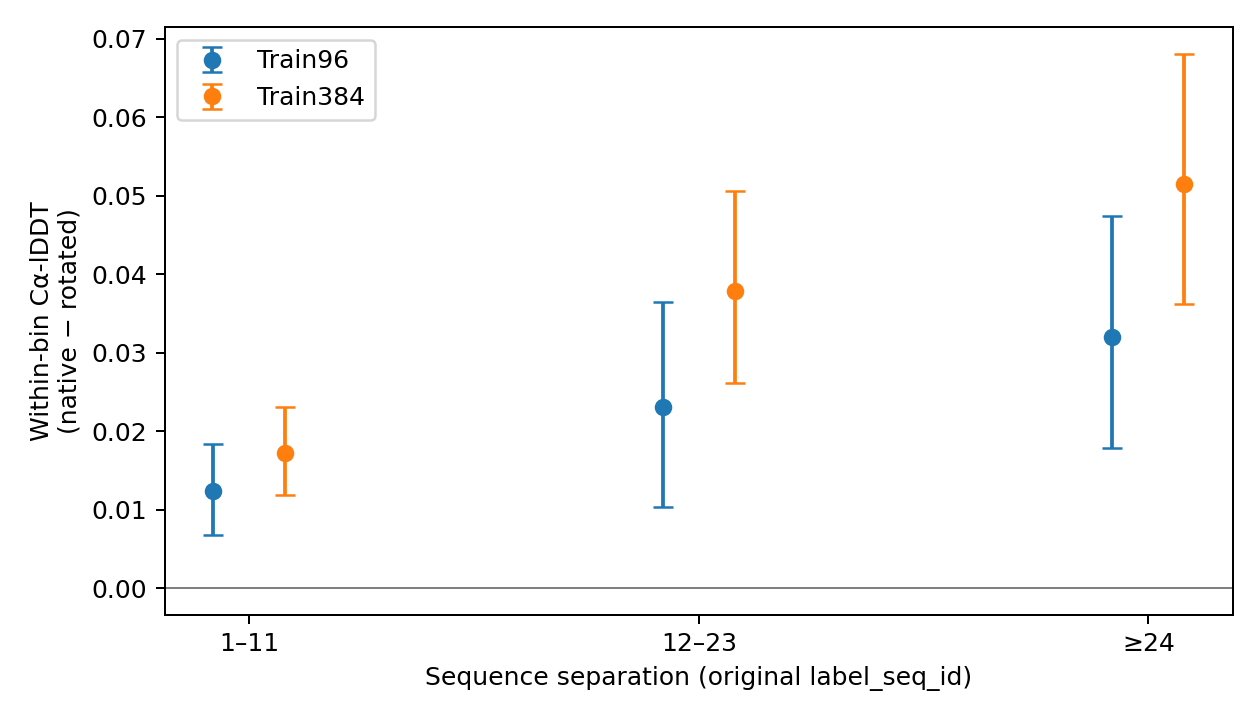
\includegraphics[keepaspectratio]{figures/score.png}}
\caption{Sequence-distance scores}
\end{figure}

\begin{figure}
\centering
\pandocbounded{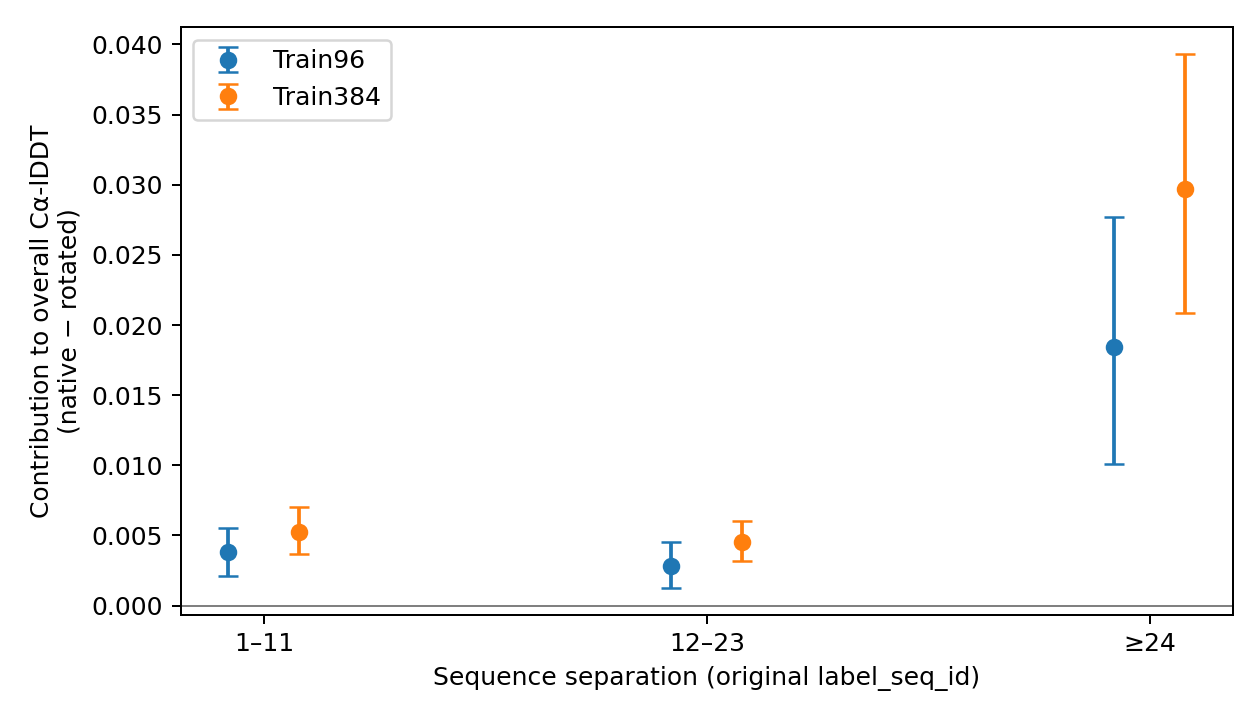
\includegraphics[keepaspectratio]{figures/contribution.png}}
\caption{Additive distance-score contributions}
\end{figure}

See the full results and exact-score audit (\nolinkurl{reports/finite_transfer_structure_20260920/structure/results.md})
and independent local verification (\nolinkurl{reports/finite_transfer_structure_20260920/structure/local_verification.json}).

\section{Finite shared parameter displacement: observed Train8→Dev8 diagnostic}\label{finite-shared-parameter-displacement-observed-train8dev8-diagnostic}

This separately locked study tests actual finite responses rather than reopening
the original derivative gate. For each of three initializations and four writer
orientations, a unit negative gradient direction is formed by averaging the
three sealed noise conditions within each training chain and then averaging
Train8 equally. Dev gradients and labels do not determine this direction or
its scale. Only the zero-initialized final Linear(256,64), with 16,448 parameters,
is displaced; all other writer and backbone parameters remain unchanged.

The inherited training-only scale is α₀=0.0003432436552346416. Independent
displacements of +10α₀, +30α₀, +100α₀, and -30α₀ are applied from the common
zero state, with +30 the sole primary node. There is no optimizer trajectory.
Each of 16 targets uses three saved noise conditions and all 12 writer
instances: 2,304 responses and 48 common baselines. The first three query-only
recycle states are fixed, and only the fourth OPM update changes. Dynamic atom
correspondence and rigid alignment are recomputed. All predictions, actual
mapping indices, random conditions and loss components are retained.

The response is r=(L₀-Lpost)/L₀, a fractional decrease of the native task loss,
not lDDT. Noise, initialization and rotation are averaged within chains;
20,000 bootstrap draws (seed 20261204) resample the eight chains of each group.
The interval conditions on the chosen training collection, shared update,
initializations and repeatedly observed development targets.

\begin{longtable}[]{@{}
  >{\raggedright\arraybackslash}p{(\linewidth - 4\tabcolsep) * \real{0.2727}}
  >{\raggedleft\arraybackslash}p{(\linewidth - 4\tabcolsep) * \real{0.3636}}
  >{\raggedleft\arraybackslash}p{(\linewidth - 4\tabcolsep) * \real{0.3636}}@{}}
\toprule\noalign{}
\begin{minipage}[b]{\linewidth}\raggedright
Group / scoring precision
\end{minipage} & \begin{minipage}[b]{\linewidth}\raggedleft
Native r
\end{minipage} & \begin{minipage}[b]{\linewidth}\raggedleft
Native-rotation
\end{minipage} \\
\midrule\noalign{}
\endhead
\bottomrule\noalign{}
\endlastfoot
Train8 / FP32 & 2.2542×10⁻⁴ {[}1.5890×10⁻⁴, 2.9052×10⁻⁴{]} & -1.8500×10⁻⁵ {[}-5.4968×10⁻⁵, 1.7494×10⁻⁵{]} \\
Dev8 / FP32 & 3.4701×10⁻⁵ {[}-1.3581×10⁻⁵, 7.6682×10⁻⁵{]} & 6.6098×10⁻⁶ {[}-2.1483×10⁻⁵, 3.4039×10⁻⁵{]} \\
Dev8 / FP64 loss and alignment & 3.4815×10⁻⁵ {[}-1.3458×10⁻⁵, 7.6935×10⁻⁵{]} & 6.6335×10⁻⁶ {[}-2.1503×10⁻⁵, 3.3994×10⁻⁵{]} \\
\end{longtable}

At +30, native loss decreases on seven of eight Dev chains, whereas the
native-rotation contrast is positive on five. Initialization-marginal contrasts
are 6.03×10⁻⁶, 6.42×10⁻⁶ and 7.38×10⁻⁶; rotation-marginal contrasts are
6.41×10⁻⁵, -3.99×10⁻⁵ and -4.36×10⁻⁶. This does not establish an average
transfer advantage, equivalence, or uniformly favorable behavior across rotations.
The +10 and +100 sensitivity nodes likewise do not establish either positive
native mean transfer or native superiority. They do not replace the primary.

Using ±30, define O=(L--L+)/(2L₀) and E=(2L₀-L+-L-)/(2L₀), so r+=O+E.
Native Dev8 O is 3.4868×10⁻⁵ {[}-1.3672×10⁻⁵, 7.7297×10⁻⁵{]}, and E is
-1.6723×10⁻⁷ {[}-9.2889×10⁻⁷, 8.6018×10⁻⁷{]}. These are finite odd/even
responses, not identified gradient and curvature contributions. Train8 improvement
is an in-sample positive control, not evidence of held-out transfer.

FP64 loss and alignment reuse the same FP32 predictions and dynamic mapping;
the backbone remains FP32. Mean absolute within-chain precision differences
on Dev8 are 2.80×10⁻⁷ for native r and 2.20×10⁻⁷ for its contrast. A predeclared
sensitivity subtracting each chain's absolute precision discrepancy does not
change the inference. This sensitivity is not a rigorous error bound for the
complete forward. All 203 treatment-induced correspondence changes are retained;
index changes alone are not interpreted as discontinuities. Parameters remain
frozen, cached states remain unchanged, and all prescribed responses are finite.

Equal parameter-step norms do not imply equal injection norms. At +30 on Dev8,
native relative injection norms range from 0.0102 to 0.0184, compared with
0.0113 to 0.0353 for rotations. Thus this tests the complete shared-update recipe,
not a pure equal-amplitude direction intervention. It supplies no new structure
predictions and does not explain or overturn the trained models' folding effects.

\begin{figure}
\centering
\pandocbounded{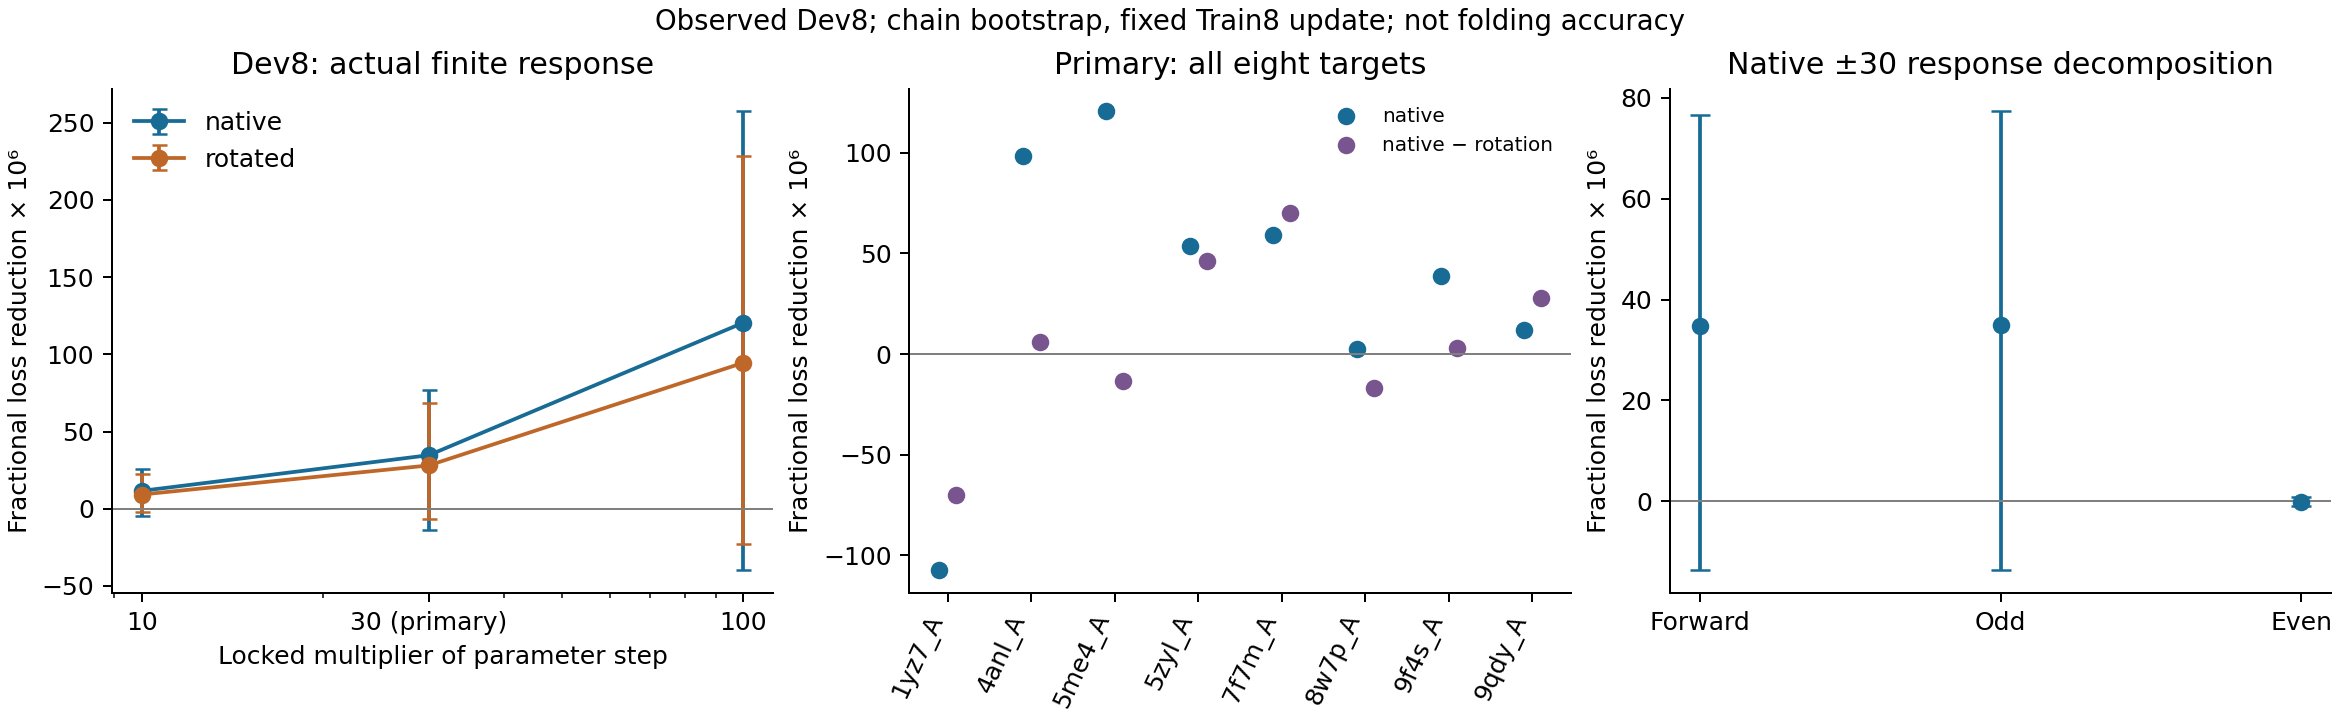
\includegraphics[keepaspectratio]{figures/response.png}}
\caption{Finite shared responses}
\end{figure}

See the locked protocol (\nolinkurl{reports/finite_transfer_structure_20260920/protocol.md}),
all fixed-node summaries (\nolinkurl{reports/finite_transfer_structure_20260920/finite/results.md}),
and completion audit (\nolinkurl{reports/finite_transfer_structure_20260920/completion_audit.json}).

The predeclared four-chain numerical subset (two training and two development
chains, all initializations/rotations/noises at ±30) is repeated in a separate
H100 process with reversed execution order and independently on each of two
W7900 cards. All three replicas contain 288 responses. The H100 repeat exactly
matches the main coordinates and both loss variants; the two W7900 copies
also agree exactly with one another. W7900 does not produce bit-identical
coordinates to H100. The largest cross-backend single-condition fractional
response difference is 5.47×10⁻⁶ (FP32 scoring), while the largest difference
in the four chain-averaged native-rotation contrasts is 3.87×10⁻⁷. The paired
noise tensors, sigma tensors, model/feature inputs and audited runtime sources
match across machines. These are bounded numerical checks, not independent
biological replication or a complete Dev8 cross-backend evaluation; see the
replica audit (\nolinkurl{reports/finite_transfer_structure_20260920/replica_audit.json}).

\section{Frozen explicit-access comparison on the observed panel}\label{frozen-explicit-access-comparison-on-the-observed-panel}

After completing the finite-transfer study, we froze the six previously selected
Train24/384-step Factor and G+ checkpoints (seeds20260920/21/22; respective
learning rates5e-5 and1e-4). The new protocol performs no training or selection.
All96 Confirm96-B targets are evaluated with seed101,c4/s5,sample0,FP32 and
the existing sequence-only evidence-read guard. Checkpoint, feature provenance,
manifest and inference source hashes are locked before prediction. Known
development-target replays for both heads match their historical CIF hashes
and all1536 atom coordinates exactly. All576 panel predictions succeed.

\begin{longtable}[]{@{}
  >{\raggedright\arraybackslash}p{(\linewidth - 8\tabcolsep) * \real{0.1579}}
  >{\raggedleft\arraybackslash}p{(\linewidth - 8\tabcolsep) * \real{0.2105}}
  >{\raggedleft\arraybackslash}p{(\linewidth - 8\tabcolsep) * \real{0.2105}}
  >{\raggedleft\arraybackslash}p{(\linewidth - 8\tabcolsep) * \real{0.2105}}
  >{\raggedleft\arraybackslash}p{(\linewidth - 8\tabcolsep) * \real{0.2105}}@{}}
\toprule\noalign{}
\begin{minipage}[b]{\linewidth}\raggedright
Metric
\end{minipage} & \begin{minipage}[b]{\linewidth}\raggedleft
Factor
\end{minipage} & \begin{minipage}[b]{\linewidth}\raggedleft
G+
\end{minipage} & \begin{minipage}[b]{\linewidth}\raggedleft
Paired difference {[}95\% target interval{]}
\end{minipage} & \begin{minipage}[b]{\linewidth}\raggedleft
Positive targets
\end{minipage} \\
\midrule\noalign{}
\endhead
\bottomrule\noalign{}
\endlastfoot
Cα pair-lDDT & 0.55314 & 0.50084 & +0.05230 {[}0.03553,0.06983{]} & 71/96 \\
Residue-averaged Cα-lDDT & 0.55113 & 0.50124 & +0.04989 {[}0.03398,0.06646{]} & 69/96 \\
Fixed-correspondence TM-score & 0.55015 & 0.49474 & +0.05541 {[}0.03413,0.07742{]} & 66/96 \\
\end{longtable}

Seeds are averaged within targets before20,000 target bootstrap draws, seed
20260927. Intervals condition on the fixed models; secondary intervals are
unadjusted. An independent AlphaFold implementation reproduces every primary
score within1.17e-14. TM-score uses the pinned executable and full query length.
The observed panel is not a new blind confirmation; the width and selected
learning-rate differences remain part of this frozen comparison. No claim about
the isolated information-access effect, optimal convergence or compute speedup
is made. Protocol and results (\nolinkurl{reports/access_panel_followup_20260920/metric_analysis/results.md}).

\section{Pair prevalence and score headroom}\label{pair-prevalence-and-score-headroom}

The original Train24 tangent direction comparison is additionally decomposed
using all1152 existing CIFs. Original label\_seq\_id bins1--11,12--23,≥24 and
reference distance\textless15Å remain fixed; every overall score reconstructs within
1e-12. Its within-bin differences are +0.03167 {[}0.02392,0.04015{]},
+0.06327 {[}0.04547,0.08208{]}, and +0.06951 {[}0.05114,0.08881{]}. The additive
contributions are +0.00966,+0.00832,+0.03912, summing to+0.05710271.

For each target and bin, let w be its share of eligible reference pairs. We
report C=mean{[}w(S\_native-S\_rotated){]} and H=mean{[}w(1-S\_rotated){]}. C/H is a
descriptive fraction of the control's remaining score space, not attainable
recovery or causal attribution. All quantities average seeds and rotations
within target first. The pair-share column averages target-specific shares;
it is not a pooled-pair weighting of the dataset.

\begin{longtable}[]{@{}
  >{\raggedright\arraybackslash}p{(\linewidth - 14\tabcolsep) * \real{0.1000}}
  >{\raggedright\arraybackslash}p{(\linewidth - 14\tabcolsep) * \real{0.1000}}
  >{\raggedleft\arraybackslash}p{(\linewidth - 14\tabcolsep) * \real{0.1333}}
  >{\raggedleft\arraybackslash}p{(\linewidth - 14\tabcolsep) * \real{0.1333}}
  >{\raggedleft\arraybackslash}p{(\linewidth - 14\tabcolsep) * \real{0.1333}}
  >{\raggedleft\arraybackslash}p{(\linewidth - 14\tabcolsep) * \real{0.1333}}
  >{\raggedleft\arraybackslash}p{(\linewidth - 14\tabcolsep) * \real{0.1333}}
  >{\raggedleft\arraybackslash}p{(\linewidth - 14\tabcolsep) * \real{0.1333}}@{}}
\toprule\noalign{}
\begin{minipage}[b]{\linewidth}\raggedright
Setting
\end{minipage} & \begin{minipage}[b]{\linewidth}\raggedright
Separation
\end{minipage} & \begin{minipage}[b]{\linewidth}\raggedleft
Pair share
\end{minipage} & \begin{minipage}[b]{\linewidth}\raggedleft
Native
\end{minipage} & \begin{minipage}[b]{\linewidth}\raggedleft
Rotated
\end{minipage} & \begin{minipage}[b]{\linewidth}\raggedleft
C
\end{minipage} & \begin{minipage}[b]{\linewidth}\raggedleft
H
\end{minipage} & \begin{minipage}[b]{\linewidth}\raggedleft
C/H
\end{minipage} \\
\midrule\noalign{}
\endhead
\bottomrule\noalign{}
\endlastfoot
Train24 tangent/384 & 1--11 & 30.41\% & 0.74641 & 0.71473 & 0.00966 & 0.08584 & 11.25\% \\
& 12--23 & 12.19\% & 0.50570 & 0.44243 & 0.00832 & 0.06748 & 12.33\% \\
& ≥24 & 57.40\% & 0.42317 & 0.35366 & 0.03912 & 0.37189 & 10.52\% \\
Train96 full/1536 & 1--11 & 30.41\% & 0.78395 & 0.77157 & 0.00379 & 0.06871 & 5.51\% \\
& 12--23 & 12.19\% & 0.58954 & 0.56652 & 0.00281 & 0.05199 & 5.40\% \\
& ≥24 & 57.40\% & 0.53254 & 0.50056 & 0.01846 & 0.28782 & 6.41\% \\
Train384 full/1536 & 1--11 & 30.41\% & 0.78621 & 0.76903 & 0.00525 & 0.06951 & 7.55\% \\
& 12--23 & 12.19\% & 0.59990 & 0.56203 & 0.00456 & 0.05259 & 8.68\% \\
& ≥24 & 57.40\% & 0.54519 & 0.49371 & 0.02970 & 0.29169 & 10.18\% \\
\end{longtable}

All96 targets have eligible pairs in each group. The ordering of headroom
ratios differs between configurations, despite positive long-range score
effects throughout. These tables support benefits on sequence-distant spatial
neighbors, without establishing a general long-range specialization or
evolutionary covariance recovery. Full precision records (\nolinkurl{reports/access_panel_followup_20260920/headroom/analysis.json}).

\section{Length48 v2: prospective adaptation-length extrapolation}\label{length48-v2-prospective-adaptation-length-extrapolation}

The fixed Mini Train384 full-factor adapters were trained on chains of 152--383
residues. A new prospective panel evaluates their complete-sequence predictions
beyond that range, without additional training. Length48 v2 contains 48 chains,
16 in each selection bin 385--512, 513--640 and 641--768; the actual selected range
is 392--750. The experiment is sequence-screened adapter-length extrapolation,
not a test of foundation-model novelty or homologous-superfamily isolation.

\subsection{Selection versions and calibration}\label{selection-versions-and-calibration}

The original Length48 v1 selection stopped at its declared candidate cap before
forming a complete panel; its provisional targets were not scored as a smaller
evaluation panel. A subsequent filter audit identified length-dependent hits
under the old global non-gap identity rule, including shuffled controls. A
separate locked calibration of BLASTP 2.17.0 against 15,605 frozen references
produced no qualifying hits for 256 shuffled controls and recovered all 288
specified embedded-source positives. These synthetic tests establish performance
on the designed controls, not biological false-positive or false-negative rates.
The calibrated rule and new deterministic candidate ordering were frozen for v2
before selecting or scoring its targets. The original v1 stop is retained.

V2 uses single-model X-ray entries at ≤2.5Å, standard amino acids, release date
≤2021-09-30, exact entity-sequence mapping and ≥90\% reference Cα coverage. It
excludes the declared exposure PDBs/sequences and all 128 PDBs/sequences used in
the two filter-development studies. Candidates are ordered by
SHA256(\texttt{length48-v2\textbar{}target\_id}), with a cap of 1,024 examined candidates per bin
and a two-hour selection budget. All 48 targets were accepted from 67 examined:
11 mapping/coverage failures, five exposure-sequence exclusions and three
within-panel exclusions. Minimum accepted reference coverage is 90.5237\%.

Search uses BLASTP 2.17.0, BLOSUM62, gap costs 11/1, word size 3, SEG enabled,
soft masking enabled and composition-based statistics 2. Retrieval E≤10⁻³,
\nolinkurl{max_target_seqs} equal to the complete database size and no HSP cap preserve
the candidates available for filtering. A single HSP excludes a candidate when
E≤10⁻⁵, identity≥30\% over alignment columns including internal gaps, at least
50 residue--residue columns and paired-column coverage≥70\% all hold. HSPs are
not merged. For the 584 known queries and admitted panel targets, the coverage
denominator is the shorter full sequence; for historical non-query teacher rows,
it is the full candidate sequence. Thus a 200-residue exposed query embedded in
a 600-residue candidate is not retained merely because its candidate coverage
is one-third. Within-panel search augments the full database with accepted panel
entries; this changes database size slightly relative to the fixed-database
calibration. All 127 search records and 34 retrieved HSPs were independently
recomputed, and the manifest was locked before prediction.

Four CATH family-linked calibration pairs were missed in both orientations at
the retrieval threshold: 3bk5\_A/1iwm\_A, 2o6r\_A/1wwl\_A, 2rj2\_A/2wo1\_A and
4g8b\_A/3wwc\_A. None was lost by downstream coverage filtering or HSP aggregation.
Auxiliary global non-gap identities were 15.05\%, 23.30\%, 19.53\% and 17.69\%; these
are contextual observations, not the BLAST exclusion identity or an exhaustive
local-search sensitivity certificate. They document why the panel cannot be
called family-held-out. The four pairs do not define a representative denominator
for estimating a natural family-miss rate.

\subsection{Frozen inference and execution chronology}\label{frozen-inference-and-execution-chronology}

Twelve frozen Train384 full-factor checkpoints cross training seeds 20260923--25
with native and three output rotations (20261001--03), all at 1,536 updates.
Query-only and official Mini-ESM complete the 14-system comparison. Inference
uses the unchanged c4/s5, sample 0, seed 101, FP32, torch kernels, TF32 disabled,
MC dropout disabled and no MSA/templates. Adapters use frozen ESM2-35M features;
the official reference uses its own ESM2-3B route. No sequence is cropped and no
prediction is selected by reference quality.

Initial H100 checks included two pure-native replays on the known short
chain 3gxb\_A and twelve unscored long-chain smoke predictions: native, one trained
rotated control, query-only and official on 422-, 614- and 750-residue targets.
The short repeats were coordinate-exact; raw Cα RMS difference from the
historical prediction was 0.00175167Å, below the predeclared 0.05Å bound (maximum
atom displacement bound 0.2Å). All twelve long smoke predictions passed. The
formal array then ran with at most eight concurrent H100 workers.

A later boundary clarification arrived after formal launch. Scoring was explicitly
paused while two pure-rotated short-chain replays and twelve instrumented long
replays were checked. Rotated short repeats were exact, with historical RMS
0.00049060Å; all twelve long replays reproduced their original smoke coordinates
exactly. Instrumentation checked full token/PLM lengths, residue-factor and pair
dimensions, and four recycle calls. These fourteen supplemental predictions
occurred after launch and before new score opening; they are not retrospectively
classified as prelaunch gates. Scientific settings, models and targets remained
unchanged. The total is 672 formal predictions plus 28 engineering predictions,
not 700 independent evaluation observations.

All 672 formal predictions succeeded before unified scoring, with no target
replacement or failed-record omission. Every output contained finite Cα
coordinates for all query positions. Source, model, feature, manifest, report and
prediction hashes were verified. Scoring used identical reference indices across
methods; the pair-lDDT implementation agreed with the pinned independent reference
within 3.83×10⁻¹⁵. Supplementary residue-averaged lDDT uses the same reference mask;
fixed-correspondence TM-score normalizes by full query length.

\subsection{Locked analysis and secondary length groups}\label{locked-analysis-and-secondary-length-groups}

The only primary contrast averages three rotations within each seed, three seeds
within each target, and then 48 equally weighted targets. Its ordinary target
bootstrap uses 20,000 draws and seed 20260928. It was not changed to stratified
resampling after the later suggestion. Intervals condition on the frozen fitted
models; family dependence and retraining uncertainty are not accounted for by
this resampling. Length-bin and supplementary metric intervals are unadjusted.
Native/query and rotated/query mean differences are descriptive comparisons, not
additional confirmation endpoints. No claim about a monotonic length trend follows
from the three separate bin means.

\begin{longtable}[]{@{}
  >{\raggedright\arraybackslash}p{(\linewidth - 10\tabcolsep) * \real{0.1364}}
  >{\raggedleft\arraybackslash}p{(\linewidth - 10\tabcolsep) * \real{0.1818}}
  >{\raggedleft\arraybackslash}p{(\linewidth - 10\tabcolsep) * \real{0.1818}}
  >{\raggedleft\arraybackslash}p{(\linewidth - 10\tabcolsep) * \real{0.1818}}
  >{\raggedright\arraybackslash}p{(\linewidth - 10\tabcolsep) * \real{0.1364}}
  >{\raggedleft\arraybackslash}p{(\linewidth - 10\tabcolsep) * \real{0.1818}}@{}}
\toprule\noalign{}
\begin{minipage}[b]{\linewidth}\raggedright
Length bin
\end{minipage} & \begin{minipage}[b]{\linewidth}\raggedleft
Targets
\end{minipage} & \begin{minipage}[b]{\linewidth}\raggedleft
Native pair-lDDT
\end{minipage} & \begin{minipage}[b]{\linewidth}\raggedleft
Rotated pair-lDDT
\end{minipage} & \begin{minipage}[b]{\linewidth}\raggedright
Difference {[}95\% target CI{]}
\end{minipage} & \begin{minipage}[b]{\linewidth}\raggedleft
Positive targets
\end{minipage} \\
\midrule\noalign{}
\endhead
\bottomrule\noalign{}
\endlastfoot
385-512 & 16 & 0.56050 & 0.50731 & +0.05319 {[}0.02388, 0.08673{]} & 13/16 \\
513-640 & 16 & 0.52388 & 0.47816 & +0.04572 {[}0.02511, 0.06924{]} & 14/16 \\
641-768 & 16 & 0.50319 & 0.47453 & +0.02866 {[}0.01433, 0.04710{]} & 14/16 \\
\end{longtable}

All three training-seed marginal differences are positive, as are all three
rotation marginals. Supplementary metric differences are +0.04029 for
residue-averaged Cα-lDDT {[}0.02726, 0.05480{]} and +0.04782 for fixed-correspondence
TM-score {[}0.03037, 0.06704{]}. They describe the same 48 structures per system,
not new independent replications. Generic and G+ were not evaluated on this panel.

An independent aggregation reproduced all absolute means, per-target differences,
seed/rotation marginals, length-bin summaries and locked bootstrap intervals from
raw records. Full precision values, provenance, selection decisions and execution
timestamps are in the Length48 report (\nolinkurl{reports/length48_v2_20260920/results.md}),
metric records (\nolinkurl{reports/length48_v2_20260920/metric_analysis/metric_records.json}),
analysis (\nolinkurl{reports/length48_v2_20260920/metric_analysis/analysis.json}) and
final audit (\nolinkurl{reports/length48_v2_20260920/final_summary_audit.json}).
The frozen v2 specification (\nolinkurl{docs/length48_v2.md}) retains its original
pre-execution status text as protocol history; the completion report records the
subsequent authorized execution. No further training, recycle interchange or
shared-transfer step search accompanies this closure.

\section{Cross-backbone construction and execution contracts}\label{cross-backbone-construction-and-execution-contracts}

The common construction in Eq. (1) is a residual around each backbone's own
operator. It does not transplant Protenix normalization, loss, PLM replacement
or recycle semantics. A live anchor can depend on previous adapter calls;
isometry claims hold for the writer at matched incoming states, not for the
entire recurrent system after independent training.

\subsection{AF2/OpenFold}\label{af2openfold}

Official AF2 \nolinkurl{model_3_ptm} weights are loaded into OpenFold. The archived parameter
file SHA256 is \nolinkurl{b53a724294cdd46a45d530b306bced8e429ffee74a4f9a2a897551b30966c415}.
All 48 main Evoformer blocks and the structure module remain intact. The adapter
wraps only the first main block's OPM and reads its live normalized/projected
MSA factors. Query-only input has one query row and a zero-masked extra-MSA row;
no homologs or templates are supplied. The output preserves native masking,
row-count normalization and baseline affine. Residual bias cancels; no cached
Protenix factor or depth constant is used.

Adapter ESM2-35M features have 480 channels. Native and rotated full-factor
heads have 373,824 trainable parameters; G+ has 378,144 and explicit factor access.
The frozen AF2 model has no native PLM to replace. Native FAPE, distogram and
supervised torsion components carry weights 1, 0.3 and 1. Confidence and
masked-MSA losses are disabled. Full experimental-structure labels, including
atom masks and frames, are prepared separately from prediction features.

The final recycle retains gradients through the frozen downstream computation;
freezing parameters does not disable input derivatives. Non-reentrant activation
checkpointing is enabled. \nolinkurl{max_recycling_iters=3} means four trunk passes.
Prediction uses seed 20260921, no early stopping and no reference-based sample
selection. The recorded formal environment is H100, PyTorch 2.7.1/CUDA 12.8.

Train96 and Train384 each have 15 fits, all evaluated at update 1,536. Formal
initialization seeds are 20260923/24/25 and rotation seeds 20261001/02/03.
An independent development seed 20260922, 384 updates, two learning rates
(5e-5 and 1e-4), and native/first-rotation/G+ arms give six calibration fits.
Dev8 means pooled equally across the three arms select one common rate, 1e-4;
Train384 retains it. AdamW uses weight decay 0.01 and gradient clipping at 1.
There is no retrospective selection of an intermediate checkpoint.

ColabFold runs the same AF2 weight identity as a separate query-only pipeline.
Its locked path uses JAX highest matmul precision, disables bfloat16 inference,
and retains its standard float16 returned recycle state. It is not required to
be bitwise identical to PyTorch. Close panel means are pipeline consistency
information, not proof of target-wise coordinate equality. No MSA-enabled
ColabFold panel was executed in this experiment (cached MSA count is zero).

Each adaptation-size summary contains 2,448 model--target score records:
2,160 adapter records and 288 query-only/ColabFold baseline records. The baseline
records are reused across adaptation sizes; they are not fresh independent
predictions or biological replicates. Both summaries report zero scoring failures.
The formal lock is \nolinkurl{reports/cross_backbone_20260921/formal_execution_lock.json}.

\subsection{Complete AF2 contrasts}\label{complete-af2-contrasts}

The following tables retain all three metrics, including null and negative
results. CA pair-lDDT is the primary metric; residue CA-lDDT and full-query-length
fixed-correspondence TM-score audit the same structures. Confidence intervals
are target-bootstrap intervals conditional on the fitted models. Seed and
rotation marginals are arithmetic means, not independent target replicates.

\begin{longtable}[]{@{}
  >{\raggedright\arraybackslash}p{(\linewidth - 8\tabcolsep) * \real{0.2000}}
  >{\raggedright\arraybackslash}p{(\linewidth - 8\tabcolsep) * \real{0.2000}}
  >{\raggedright\arraybackslash}p{(\linewidth - 8\tabcolsep) * \real{0.2000}}
  >{\raggedright\arraybackslash}p{(\linewidth - 8\tabcolsep) * \real{0.2000}}
  >{\raggedright\arraybackslash}p{(\linewidth - 8\tabcolsep) * \real{0.2000}}@{}}
\toprule\noalign{}
\begin{minipage}[b]{\linewidth}\raggedright
Training
\end{minipage} & \begin{minipage}[b]{\linewidth}\raggedright
Panel
\end{minipage} & \begin{minipage}[b]{\linewidth}\raggedright
Metric
\end{minipage} & \begin{minipage}[b]{\linewidth}\raggedright
Native-rotation {[}95\% CI{]}
\end{minipage} & \begin{minipage}[b]{\linewidth}\raggedright
Positive targets
\end{minipage} \\
\midrule\noalign{}
\endhead
\bottomrule\noalign{}
\endlastfoot
Train96 & confirm96 & CA pair-lDDT & +0.01981 {[}+0.00928, +0.03129{]} & 59/96 \\
Train96 & confirm96 & Residue CA-lDDT & +0.01866 {[}+0.00868, +0.02953{]} & 58/96 \\
Train96 & confirm96 & TM-score & +0.01987 {[}+0.00595, +0.03509{]} & 54/96 \\
Train96 & length48 & CA pair-lDDT & +0.01038 {[}+0.00403, +0.01705{]} & 34/48 \\
Train96 & length48 & Residue CA-lDDT & +0.00952 {[}+0.00356, +0.01587{]} & 32/48 \\
Train96 & length48 & TM-score & +0.01630 {[}+0.00343, +0.02953{]} & 29/48 \\
Train384 & confirm96 & CA pair-lDDT & +0.00303 {[}-0.00675, +0.01218{]} & 50/96 \\
Train384 & confirm96 & Residue CA-lDDT & +0.00342 {[}-0.00587, +0.01215{]} & 53/96 \\
Train384 & confirm96 & TM-score & +0.00056 {[}-0.01224, +0.01290{]} & 51/96 \\
Train384 & length48 & CA pair-lDDT & +0.01126 {[}+0.00527, +0.01734{]} & 35/48 \\
Train384 & length48 & Residue CA-lDDT & +0.01090 {[}+0.00503, +0.01682{]} & 35/48 \\
Train384 & length48 & TM-score & +0.01012 {[}+0.00079, +0.02003{]} & 27/48 \\
\end{longtable}

\begin{longtable}[]{@{}
  >{\raggedright\arraybackslash}p{(\linewidth - 6\tabcolsep) * \real{0.2500}}
  >{\raggedright\arraybackslash}p{(\linewidth - 6\tabcolsep) * \real{0.2500}}
  >{\raggedright\arraybackslash}p{(\linewidth - 6\tabcolsep) * \real{0.2500}}
  >{\raggedright\arraybackslash}p{(\linewidth - 6\tabcolsep) * \real{0.2500}}@{}}
\toprule\noalign{}
\begin{minipage}[b]{\linewidth}\raggedright
Training
\end{minipage} & \begin{minipage}[b]{\linewidth}\raggedright
Panel
\end{minipage} & \begin{minipage}[b]{\linewidth}\raggedright
Pair-lDDT seed marginals
\end{minipage} & \begin{minipage}[b]{\linewidth}\raggedright
Pair-lDDT rotation marginals
\end{minipage} \\
\midrule\noalign{}
\endhead
\bottomrule\noalign{}
\endlastfoot
Train96 & confirm96 & +0.02073, +0.02901, +0.00969 & +0.01799, +0.02220, +0.01924 \\
Train96 & length48 & +0.00877, +0.01072, +0.01166 & +0.00854, +0.00824, +0.01437 \\
Train384 & confirm96 & +0.01074, -0.01428, +0.01263 & +0.00067, +0.00702, +0.00140 \\
Train384 & length48 & +0.01014, +0.00621, +0.01742 & +0.01060, +0.00610, +0.01707 \\
\end{longtable}

The following supplementary contrasts were specified after observing the main
results. They use the same complete target records, averaging paired seeds
and rotations before 20,000 target-bootstrap draws (seed 20260921). Intervals
are unadjusted for multiple comparisons. An interaction is computed directly
per target; intervals from separate contrasts are never subtracted.

\begin{longtable}[]{@{}
  >{\raggedright\arraybackslash}p{(\linewidth - 4\tabcolsep) * \real{0.3333}}
  >{\raggedright\arraybackslash}p{(\linewidth - 4\tabcolsep) * \real{0.3333}}
  >{\raggedright\arraybackslash}p{(\linewidth - 4\tabcolsep) * \real{0.3333}}@{}}
\toprule\noalign{}
\begin{minipage}[b]{\linewidth}\raggedright
Panel
\end{minipage} & \begin{minipage}[b]{\linewidth}\raggedright
Pair-lDDT contrast
\end{minipage} & \begin{minipage}[b]{\linewidth}\raggedright
Mean {[}95\% CI{]}
\end{minipage} \\
\midrule\noalign{}
\endhead
\bottomrule\noalign{}
\endlastfoot
confirm96 & train96 native minus gplus & +0.00656 {[}-0.00515, +0.01845{]} \\
confirm96 & train384 native minus gplus & -0.00648 {[}-0.01777, +0.00537{]} \\
confirm96 & direction interaction 384 minus 96 & -0.01678 {[}-0.03214, -0.00261{]} \\
confirm96 & native 384 minus 96 & +0.00494 {[}-0.00759, +0.01779{]} \\
confirm96 & rotated 384 minus 96 & +0.02172 {[}+0.01429, +0.02942{]} \\
confirm96 & gplus 384 minus 96 & +0.01799 {[}+0.00914, +0.02667{]} \\
length48 & train96 native minus gplus & -0.00977 {[}-0.01674, -0.00288{]} \\
length48 & train384 native minus gplus & -0.00703 {[}-0.01369, -0.00039{]} \\
length48 & direction interaction 384 minus 96 & +0.00087 {[}-0.00728, +0.00863{]} \\
length48 & native 384 minus 96 & +0.01293 {[}+0.00454, +0.02223{]} \\
length48 & rotated 384 minus 96 & +0.01206 {[}+0.00534, +0.01955{]} \\
length48 & gplus 384 minus 96 & +0.01019 {[}+0.00226, +0.01904{]} \\
\end{longtable}

The full three-metric post-result arrays and source hashes remain in
\nolinkurl{reports/openfold_followup_20260921/paired_analysis.json}. The main text reports
the primary-score contrasts rather than selecting whichever metric favors a
particular adapter. AF2 does not support universal native-head superiority.

\subsection{AtlasFold non-OPM extension: locked, incomplete adaptation study}\label{atlasfold-non-opm-extension-locked-incomplete-adaptation-study}

The pinned source is \nolinkurl{8ab3aca0e18c8b814d5ca6756b2617a07d72c68d}. Folding weights
\nolinkurl{atlasfold-260703.pth} have SHA256
\nolinkurl{cbadb227d40e801a3d268d6e884e6ed3c6b9fb89d558739fcf5970492732e5ea};
AtlasLM-3B weights have SHA256
\nolinkurl{8097cc4a234853f19ca97435844829d84fe7f13215c900e74659fa9682cc0ddb}.
The native AtlasLM is retained. Its approximately 3B parameters are not omitted
when describing full-system resource requirements.

The selected site is \nolinkurl{lm_stack.blocks.0.pairwise_prod_diff}. Live factors are
formed by \nolinkurl{linear_in(layernorm(s))}, with factor dimension 128. The native map
concatenates difference first, product second: \texttt{{[}a\_i-b\_j;\ a\_i*b\_j{]}}, then applies
the frozen output affine. The residual includes the two cross-products and the
quadratic increment product. It cancels the output bias and does not introduce
OPM normalization. Native/rotation heads have 423,168 trainable parameters;
G+ has 415,008. These counts are measured from the instantiated heads.

Training uses native distogram weight 0.4 and diffusion weight 2; the latter
contains weighted MSE and smooth-lDDT with internal weights 1. Confidence is
disabled. BF16 autocast is used with FP32 diffusion/loss; stochastic dropout is
off, but native MLM/noise conditioning remains. Full entity sequences, original
unresolved atom14 masks and padding to a multiple of four are retained.
No low-coverage chain is dropped from the locked Train96/Dev8 inventory.

The training call has \nolinkurl{num_recycles=3} (four trunk passes). Inference passes
\nolinkurl{num_recycles=4}; the pinned loop \nolinkurl{range(0,\ num_recycles+1)} executes five trunk
passes. The original length rule uses 20 diffusion steps through length 512,
30 through 1024, one sample, seed 1 and MLM probability 0.15. No structure score
is used to select an output or inference budget.

The 15-fit matrix uses Train96/1,536 updates and the same formal/rotation seeds
listed for AF2. Six symmetric development calibration fits selected common
learning rate 1e-4. The primary comparison is native-rotation on observed
Confirm96-B; Length48 and G+ comparisons are secondary. No final adapter-effect
estimate is reported while this matrix is incomplete. Positive, null and
negative outcomes fill the same reserved table and retain all seed marginals.

Engineering history is separate from model-quality evidence. A local compatibility
patch changes two in-place triangle-attention query scalings to out-of-place
multiplication; component forwards are exactly equal and gradients are finite.
Early label/window preflight revisions are preserved in the v1/v2/v3 locks.
In the first formal evaluation batch, transferred absolute symlinks caused
reference/feature FileNotFoundError records. A logged repair validates all 144
reference hashes and 144 full-length ESM feature entries. Original failure
records are retained; a separately named recovery evaluation reuses existing
valid CIFs and fixed final checkpoints, and generates missing predictions.
The eventual summary must identify recovered records and retain the original
engineering ledger. This does not authorize checkpoint selection, cropping,
target replacement or deletion of genuine model prediction failures.

The v3 execution-lock SHA256 is
\nolinkurl{7369e40024b70097401b4e8f0e2e0d664e78022cefa844c3ea0afdf7d8f4be17}.
Completed original AtlasFold system references below are independent of the
unfinished adapter comparison.

\section{Original-system references and execution scope}\label{original-system-references-and-execution-scope}

All rows below use the same 96+48 complete target sequences, one retained
prediction per model/target and no supplied homologs or templates. They are
descriptive system references, not a cross-model direction experiment or a
matched-compute leaderboard. Source/weight choice, PLM capacity, training
exposure and native sampling budgets differ.

\begin{longtable}[]{@{}llrrr@{}}
\toprule\noalign{}
Original system & Panel & Pair-lDDT & Residue CA-lDDT & TM-score \\
\midrule\noalign{}
\endhead
\bottomrule\noalign{}
\endlastfoot
AtlasFold & confirm96 & 0.95676 & 0.95034 & 0.93476 \\
AtlasFold & length48 & 0.95050 & 0.94429 & 0.93180 \\
OpenFold3 / OpenBind-0 & confirm96 & 0.36091 & 0.37193 & 0.33557 \\
OpenFold3 / OpenBind-0 & length48 & 0.30814 & 0.32603 & 0.26151 \\
RF3 Benchmark & confirm96 & 0.41558 & 0.42151 & 0.39250 \\
RF3 Benchmark & length48 & 0.34672 & 0.35757 & 0.29936 \\
\end{longtable}

OpenFold3 framework commit \nolinkurl{7de748b7bc93adb5af0a4032d5e9f208b6e1325f} runs
OpenBind-0 \nolinkurl{of3-ob-2025-06-30-174k.pt}, SHA256
\nolinkurl{bd43301c011d5f87580d3e8b548658869433e4488399feb03035ba248f8e29e4}.
The fixed prediction YAML SHA256 is
\nolinkurl{56dcd6b7fb4b87692a150351f2cfafed413e31818fb4b4165a23aec27c2a7980};
seed 1 and one sample are used with the native Torch backend. The framework
and parameter set are named separately; this is not a trained adapter result.
The fully resolved preset should accompany the submission artifact rather than
being inferred from another AF3-style system's budget.

RF3 uses Benchmark weights, SHA256
\nolinkurl{922901088366abb6e001bc5bd304f4002667fa7eb379cd901c94e4cac0bff762},
source commit \nolinkurl{b02eed6a6bdf8f44d14a80cc36e3da13c9f2291c}, 10 recycles,
50 sampling steps, one sample, seed 1 and no early stop. The execution path uses
native Torch with \nolinkurl{DISABLE_CUEQUIVARIANCE=1}. Neither RF3 nor OpenFold3 has a
completed native-rotation adapter matrix in this report.

ESMFold2 remains pending complete scoring; no partial-target mean is inserted
into the comparison. Its locked route retains full ESMC-6B and uses 20 loops,
100 steps and one sample. Transient HIP failures are retried with completed,
hash-validated predictions reused and failed launches retained; retries do not
constitute additional biological samples or independent validations.

Cross-system peak-memory and end-to-end timing aggregation is not yet complete.
We therefore make no new cost-superiority claim. The earlier Protenix stage
measurements in Appendix D keep their original exclusions and hardware scope.
System quality cannot be normalized by the adapter's parameter count alone.
